
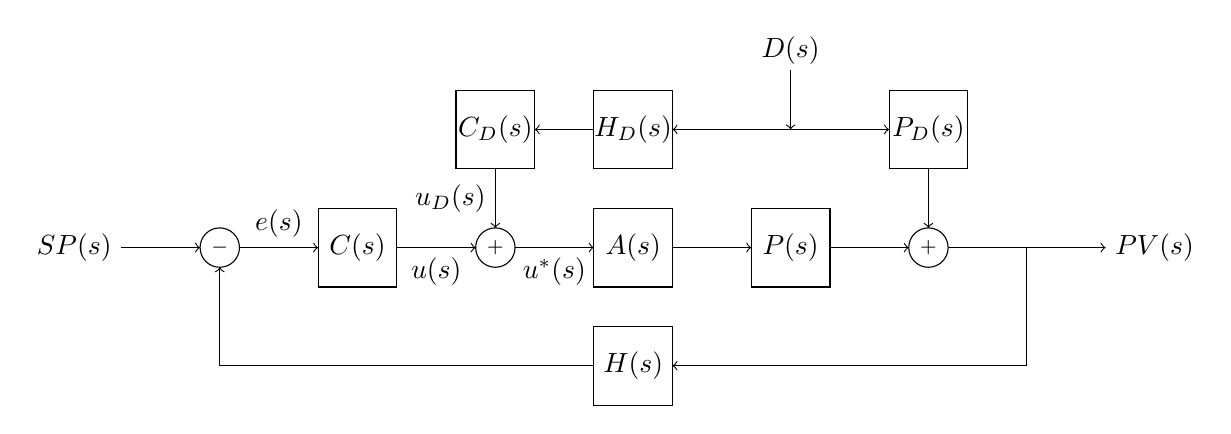
\begin{tikzpicture}
    
    %Error Sum
    \draw[->] (-4.5,0) node[anchor=east]{$SP(s)$}-- (-3.5,0);
    \draw (-3.25,0) circle (0.25) node{\scriptsize$-$};
    %Controller
    \draw[->] (-3,0) -- (-2,0)node[pos=0.5,anchor=south]{$e(s)$};
    \draw (-2,-0.5) rectangle (-1,0.5) node[pos=0.5]{$C(s)$};
    \draw[->] (-1,0) -- (0,0) node[pos=0.5,anchor=north]{$u(s)$};
    %Control Sum
    \draw (0.25,0) circle (0.25) node{\scriptsize$+$}; 
    %Actuator
    \draw[->] (0.5,0) -- (1.5,0)node[pos=0.5,anchor=north]{$u^*(s)$};
    \draw (1.5,-0.5) rectangle (2.5,0.5) node[pos=0.5]{$A(s)$};
    \draw[->] (2.5,0) -- (3.5,0);
    %Process
    \draw (3.5,-0.5) rectangle (4.5,0.5) node[pos=0.5]{$P(s)$};
    \draw[->] (4.5,0) -- (5.5,0);
    \draw[->] (6,0) -- (8,0)node[anchor=west]{$PV(s)$};
    %Output Sum
    \draw (5.75,0) circle (0.25) node{\scriptsize$+$};
    %Transducer
    \draw[->] (7,0) -- (7,-1.5) -- (2.5,-1.5);
    \draw (1.5,-2) rectangle (2.5,-1) node[pos=0.5]{$H(s)$} ;
    \draw[->] (1.5,-1.5) -- (-3.25,-1.5) -- (-3.25,-0.25);
    %Disturbance Transducer
    \draw (1.5,1) rectangle (2.5,2) node[pos=0.5]{$H_D(s)$} ;
    \draw[->] (1.5,1.5) -- (0.75,1.5);
    %Disturbance Controller
    \draw (-0.25,1) rectangle (0.75,2) node[pos=0.5]{$C_D(s)$};
    \draw[->] (0.25,1) -- (0.25,0.25)node[pos=0.5,anchor=east]{$u_D(s)$};
    %Disturbance Dynamics
    \draw (5.25,1) rectangle (6.25,2) node[pos=0.5]{$P_D(s)$};
    \draw[->] (5.75,1) -- (5.75,0.25);
    %Disturbance
    \node at (4,2.5) {$D(s)$};
    \draw[<->] (2.5,1.5) -- (5.25,1.5);
    \draw[->] (4,2.25) -- (4,1.5);
\end{tikzpicture}
